% lfw.tex
%
% Author       : James Mnatzaganian, Qutaiba Saleh
% Date Created : 05/04/15
%
% Description  : LFW Paper
%
% Copyright (c) 2014 NanoComputing Research Lab

% Define the document type
\documentclass[10pt,journal]{IEEEtran}

% Packages
\usepackage{cite}
\usepackage[hidelinks]{hyperref}
\usepackage{graphicx}
\usepackage{amsmath}
\usepackage{fixltx2e}

% Package configuration
\graphicspath{{figures/}}

% Macros
\newcommand{\fig}[1]{Fig.~\ref{#1}}
\newcommand{\eq}[1]{(\ref{#1})}

% Add DRAFT to the document
\usepackage{watermark}
\watermark{\hspace{-0.3in} \textbf{DRAFT} \hspace{2.0in} \textbf{\today}}

\begin{document}
	
	\title{An Efficient Hardware Implementation of Competitive Learning Classifier for Gender Classification}
	
	\author{
		James~Mnatzaganian,~\IEEEmembership{Student Member,~IEEE,}
        and~Qutaiba~Saleh,~\IEEEmembership{Student Member,~IEEE,}%
	
		\IEEEcompsocitemizethanks{
			\IEEEcompsocthanksitem J. Mnatzaganian, and Q. Saleh are with the NanoComputing Research Laboratory, Rochester Institute of Technology, Rochester, NY, 14623.
		}%
		
		% \thanks{Manuscript received ? ?, 2015.}
	}
	
	% \markboth{Journal of IEEE Transactions,~Vol.~?, No.~?, ?~2015}%
	
	\IEEEtitleabstractindextext{%
		\begin{abstract}
			TEXT
		\end{abstract}
	
	\begin{IEEEkeywords}
		?, ?, ?.
	\end{IEEEkeywords}}

	\maketitle
	\IEEEdisplaynontitleabstractindextext
	
	\IEEEPARstart{I}{ntroduction}
		TEXT
	
	\subsection{Dataset}
		The Labeled Faces in the Wild (LFW)~\cite{lfw} dataset was modified for use with gender classification. This dataset is comprised of one or more faces per person, with no labels to denote gender. To obtain the genders, the genderize.io~\cite{genderize} API was utilized. This API can be used to obtain the gender, with a confidence interval, for a given first name. Only results with over 90\% accuracy were utilized.
		
		The faces in the dataset are not all frontalized nor are they cropped to remove background noise. To remove noise, the frontalized images from Hassner et al.~\cite{frontalize} were used as the dataset. This dataset frontalized and cropped all images from the LFW dataset, creating a cleaner dataset.
		
		To ensure that the dataset would not be biased towards a particular individual, a single instance of each person was randomly chosen. The remaining images were then randomized and split by gender, to ensure an equal distribution of males and females. 400 of each gender were used for training and 200 of each gender were used for testing. All code for generating the dataset as well as the software and hardware models are available at~\cite{gitrepo}.
	
	\subsection{Design Approach}
		The primary design constraints were area and power. With this in mind, the system still had to perform its primary goal of gender classification. It was desired to obtain the highest possible accuracy; however, if a minor loss in accuracy resulted in major hardware improvements, favor was given to the hardware.
		
		\subsubsection{Algorithm}
			An algorithm similar to competitive learning was designed. This algorithm is coined Competitive Learning Classifier (CLC). The algorithm is comprised of \(n\) competitive learning networks, where \(n\) is the number of labels. Each network has \(i\) inputs and \(o\) outputs, where each output represents a cluster. The implementation of this algorithm used for this work is shown in \fig{fig:network}. It consists of two competitive learning networks (one for males and one for females), 49 inputs per network (one for each feature), and a single cluster for the output of each network.
			
			In CLC, there is a randomly initialized weight for each input in each network. The weights are updated using the online update equation in \eq{weight_update}, where \(w_{i,n}\) is the weight of input \(i\) for network \(n\), \(\alpha\) is the learning rate, \(\hat{y}_{o,n}^{(p)}\) is output \(o\) of network \(n\) for pattern \(p\), and \(u_i^{(p)}\) is input \(i\) for pattern \(p\). Each output is computed by finding the squared Euclidean distance between the weight and the input. The corresponding cost function is shown in \eq{cost_function}, where \(P\) is the total number of patterns and \(O\) is the total number of outputs.
			
			If \(O>1\) dead neurons may occur. To combat this, boosting is used, where frequently winning neurons are negatively boosted and infrequently winning neurons are positively boosted. Boosting is only updated during the learning phase, so after training the boost values are fixed.
			
			Training occurs by selecting the network representing the current label and updating its weights. The other networks are left untouched. During testing, both networks receive the same input and compute their respective outputs. The neuron having the lowest value is the winning neuron and the network that it belongs to becomes the output of the network.
			
			\begin{figure}
				\centering
				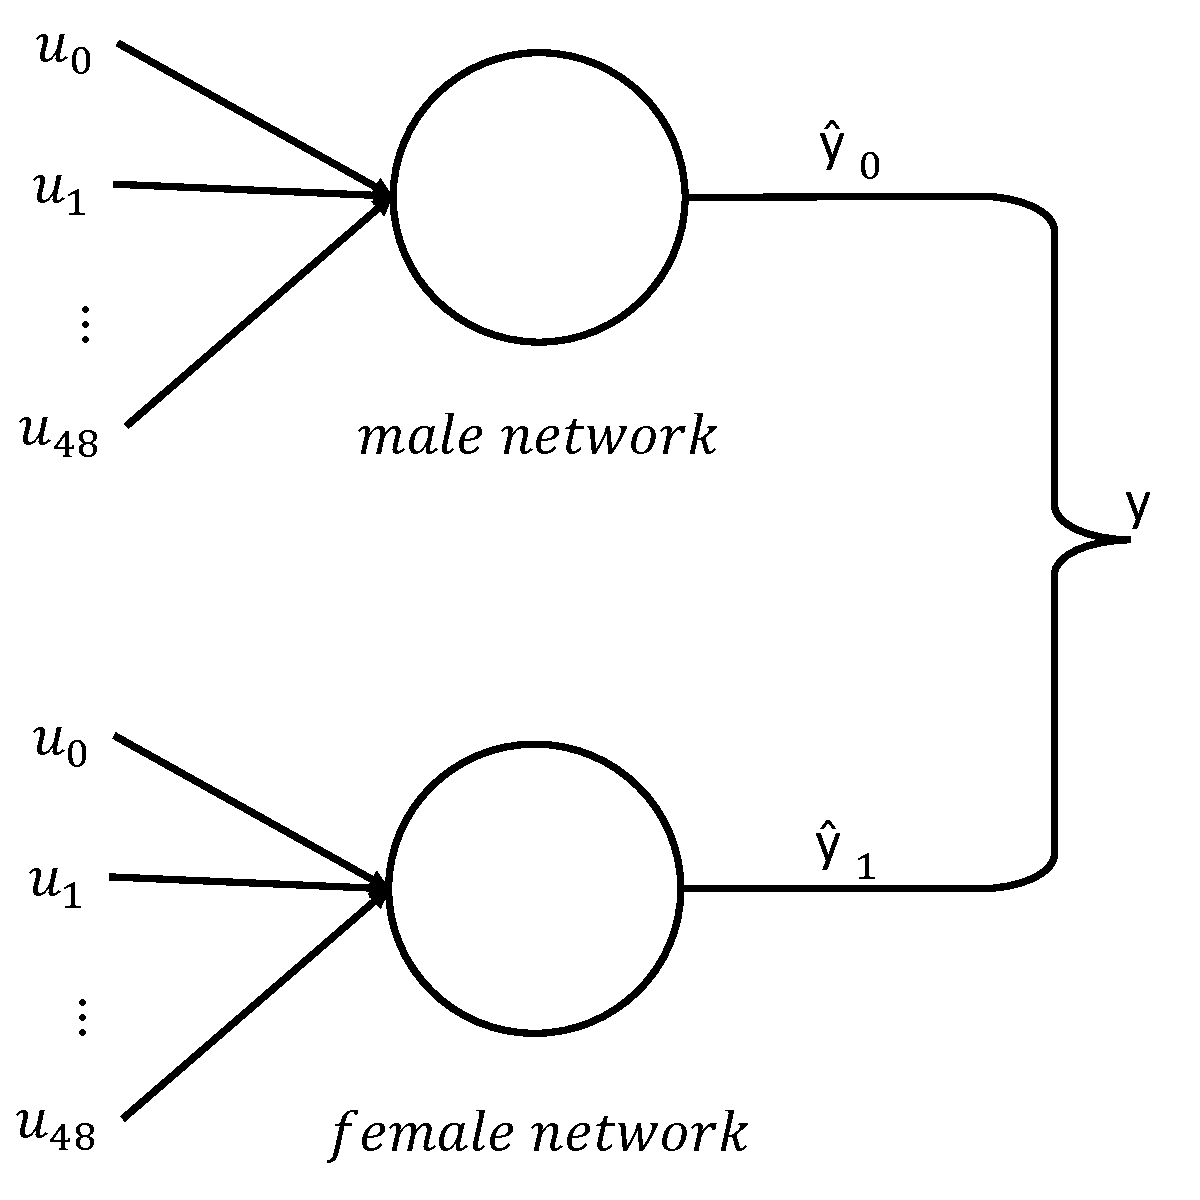
\includegraphics[width=0.8\linewidth]{network}
				\caption{A CLC consisting of two networks (male and female), 49 inputs per network, and a single output for each network.}
				\label{fig:network}
			\end{figure}
			
			\begin{equation}
				\label{weight_update}
				w_{i,n} \mathrel{+}= \alpha\hat{y}_{o,n}^{(p)}(u_i^{(p)}-w_{i,n})
			\end{equation}
			
			\begin{equation}
				\label{cost_function}
				J(\boldsymbol{w}_n) = \cfrac{1}{2}\displaystyle\sum_{p=1}^{P}\displaystyle\sum_{o=1}^{O}\hat{y}_{o,n}^{(p)}|\boldsymbol{w}_n-\boldsymbol{u}^{(p)}|^2
			\end{equation}
		
		\subsubsection{Software}
			TEXT
		
		\subsubsection{Hardware}
			TEXT
	
	\subsection{Results}
		TEXT
	
	\section{Conclusion}
		TEXT
	
	% Bibliography
	\bibliographystyle{IEEEtran}
		\bibliography{IEEEabrv,lfw}
	
\end{document}